\documentclass[oneside,12pt]{scrartcl}
\usepackage[utf8]{inputenc}
\usepackage{graphicx}
\usepackage{eso-pic}
\usepackage{caption}
\usepackage{subcaption}
\usepackage{minted}
\usepackage{parskip}
\usepackage{xcolor}
\usepackage{silence}
\usepackage[hidelinks]{hyperref}
\usepackage{arydshln}
\usepackage{algorithm}
\usepackage{algorithmic}

\newcommand*{\escape}[1]{\texttt{\textbackslash#1}}
\newcommand{\insererText}{\textcolor{red}{[INSERER TEXTE ICI]}}
\newcommand{\insererTextT}[1]{\insererText\ \textcolor{red}{#1}}
\newcommand{\insererImage}{\textcolor{red}{[INSERER IMAGE ICI]}}
\newcommand{\HRule}{\rule{\linewidth}{0.5mm}} % Defines a new command for the horizontal lines, change thickness here


\renewcommand{\thesection}{\Roman{section}} %redefini apparence nom sections (affichage chiffres romains)



\begin{document}

\begin{titlepage}

\center % Center everything on the page

%----------------------------------------------------------------------------------------
%	TITLE SECTION
%----------------------------------------------------------------------------------------

%\HRule \\[0.4cm]
%{ \huge \bfseries Interaction between Artificial Intelligence and Computer Architecture}\\[0.4cm] % Title of your document
%\HRule \\[1.5cm]

\HRule \\[0.4cm]
{ \huge \bfseries Protocole 2D-Doc et Algorithmes}\\[0.4cm] % Title of your document
%{ \huge \bfseries Leveraging Artificial Intelligence Algorithms \\ to Design Hardware Prediction Mechanisms}\\[0.4cm] % Title of your document
\HRule \\[1.5cm]

\textsc{\huge \textbf{Documentation Technique}}\\[1.5cm]

\textsc{\Large \textbf{Université de Rouen Normandie \\[0.07cm] UFR des Sciences et Technique \\[1,5cm] Master 1 Informatique\\[0.5cm] Projet Datamatrix M1 SSI 2021-2022}}


%----------------------------------------------------------------------------------------
%	AUTHOR & ADVISOR(S) SECTION
%----------------------------------------------------------------------------------------

\vspace{3cm}

\begin{center} \large
\Large \emph{Auteur:}\\[0.1cm]
\large BELABDOUN Billal\\
\end{center}
\vspace{1cm}

%----------------------------------------------------------------------------------------
%	DATE SECTION
%----------------------------------------------------------------------------------------

{\large Mai 2022}\\[1cm]
%----------------------------------------------------------------------------------------

\vfill % Fill the rest of the page with whitespace

\end{titlepage}

\thispagestyle{empty} %pour retirer la 1ere page de la pagination

\newpage

\begin{center}
\textsc{\Large \textbf{Révision du document}}
\end{center}
\vspace{2cm}

\begin{tabular}{|c|c|c|}
    \hline
  N° de version & Date de modification & Modifications apportées  \\
    \hline
    1.0 & 14/03/22 & Livrable 2 \\ \hline
    1.1 & 11/04/22 & Modifications suite au retour de la cliente\\  \hline
    1.1 & 18/04/22 & Modification suite à l'ajout d'une table (signature json)\\ \hline
    1.2 & 09/05/22 & Modification pour ajout de la partie technique\\ 
    \hline
\end{tabular}

\newpage
\pagenumbering{arabic} %remet la pagination pour le sommaire
{
\renewcommand*\contentsname{Sommaire}
\tableofcontents
}

\clearpage

\section{Préliminaires}

Le système d'authentification du projet \texttt{2DMatrix} permet de se connecter aux différents outils administratifs (\texttt{2DMatrix-Create} et \texttt{2DMatrix-Manage}). Il y a deux moyens de s'authentifier, soit via un compte classique login/password, soit via une authentification forte. On peut donc se connecter vers l'outil \texttt{2DMatrix-Create} avec un compte utilisateur organisme et sur \texttt{2DMatrix-Manage} avec soit un compte administrateur organisme, soit en authentification forte \texttt{SSL/TLS}. (certificat client) 

\section{Interface de Connexion}

Le système d'authentification est mis en place coté serveur en \texttt{PHP} et est utilisable avec une interface web coté client. Elle comporte un formulaire attendant, un couple login/password pour les connexions standard et un bouton cliquable en forme de certificat pour l'authentification forte \texttt{SSL/TLS}.

\begin{center}
    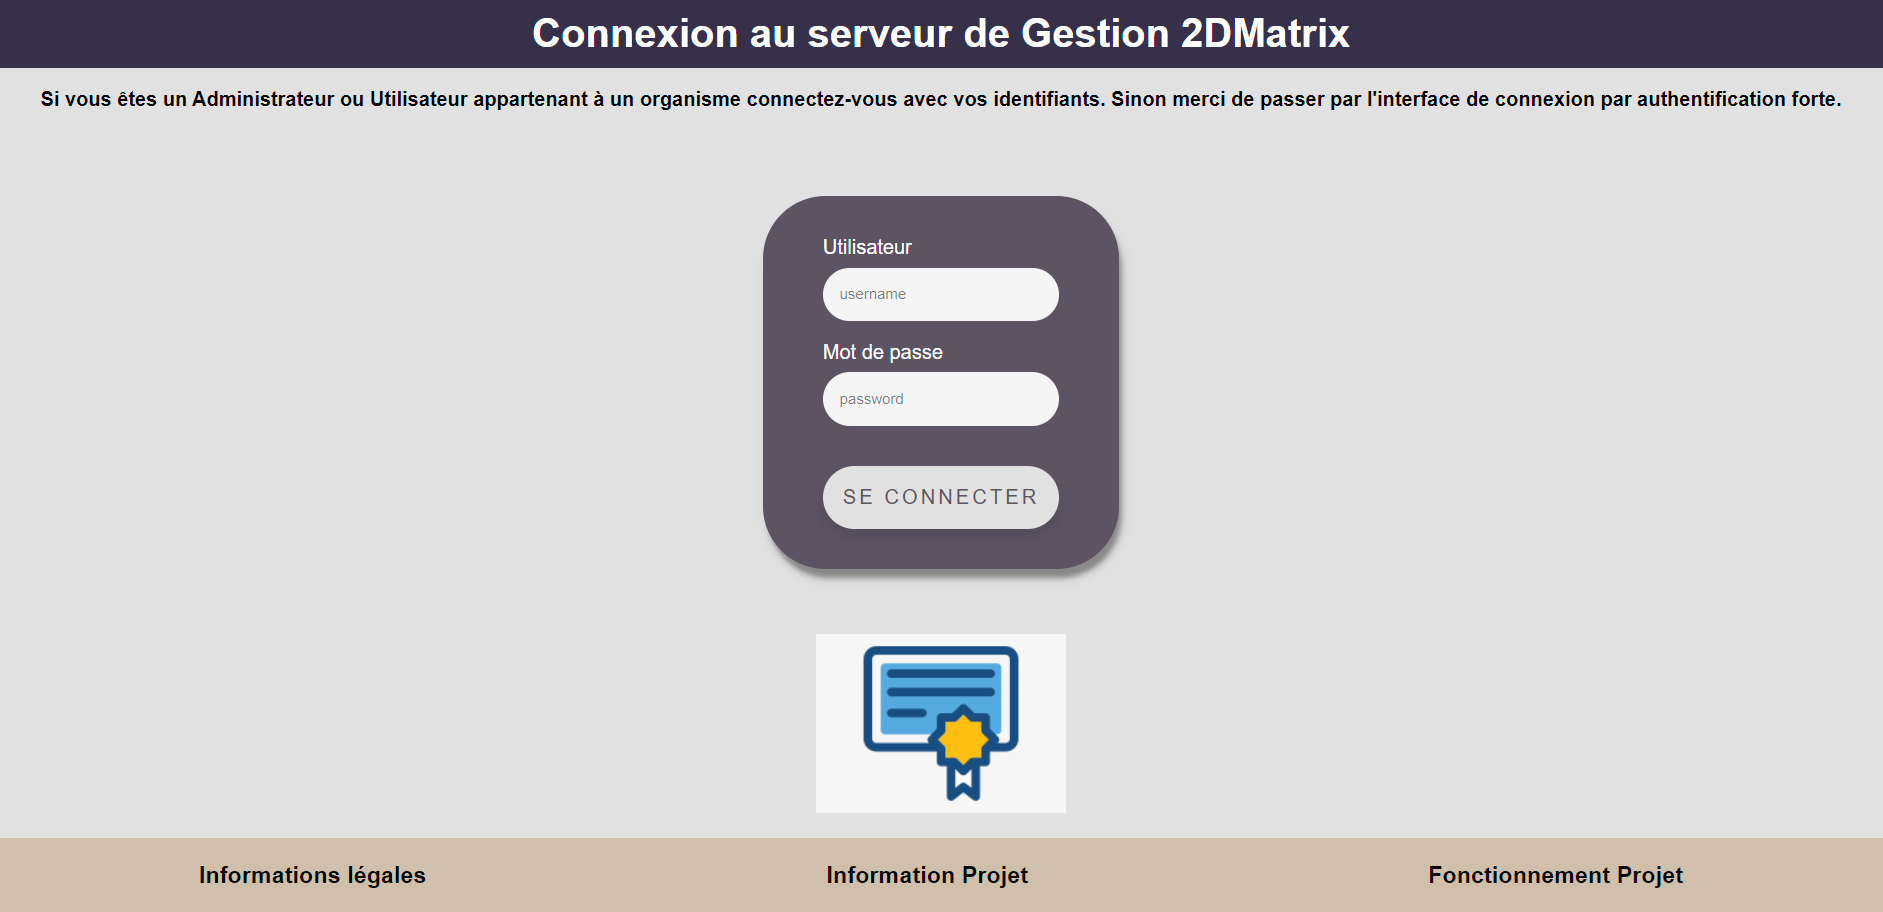
\includegraphics[scale=0.3]{imgs/authPNG.PNG}\\
    \texttt{Interface web du système d'authentification}
\end{center}

\subsection{Authentification par identifiants}

La connexion par identification login/password est géré par un formulaire \texttt{HTML} standard. Ce dernier attend les valeurs des paramètres de connexion et appelle le script \texttt{connexion.php} qui va prendre en charge les valeurs entrées via le tableau \texttt{\$\_POST}.

La connexion grâce au formulaire permet en fonction du type de compte d'accédé à la section réservé au type du compte :

\begin{itemize}
    \item utilisateur organisme : \texttt{2DMatrix-Create}
    \item administrateur organisme : \texttt{2DMatrix-Manage} section administrateur organisme.\footnote{Cette section est dynamique en fonction du compte connecté afin de permettre à l'administrateur de gérer son organisme et uniquement son organisme. Il n'aura évidemment accès à aucune donnée d'un autre organisme. }
\end{itemize}

Le script va donc récupérer les valeurs du tableau \texttt{\$\_POST} de manière sécurisé grâce à la fonction \texttt{htmlspecialchars()}. Cela permet de dé spécialiser les chaines de caractères et donc notamment d'éviter des problèmes d'injections. 

La procédure de vérification est telle que :
\begin{algorithm}
\caption{Vérification de l'authentification}
\begin{algorithmic} 
\STATE Récupération d'une connexion \texttt{PDO} à la base.
\STATE Sélection des comptes avec ce couple login/password
\IF{Compte trouvé}
\STATE Régénération de la session \texttt{PHP}
\STATE Assignement des données utiles en base vers le tableau \texttt{\$\_SESSION}
\STATE Test du type de compte (booléen)
\IF{type == 0}
\STATE Redirection vers \texttt{2DMatrix-Create} 
\ELSE
\STATE Redirection vers \texttt{2DMatrix-Manage}  
\ENDIF
\ELSE
\STATE Redirection sur l'interface avec message d'erreur
\ENDIF
\end{algorithmic}
\end{algorithm}

\subsection{Authentification Forte SSL/TLS}

En ce qui concerne l'authentification forte, il s'agit d'une vérification de certificat client. Le principe est basé sur \texttt{SSL/TLS} et permet donc de prouver que l'on est bien autorisé à accéder à un endroit sur le serveur web via un certificat venant de notre autorité racine.

\begin{center}
    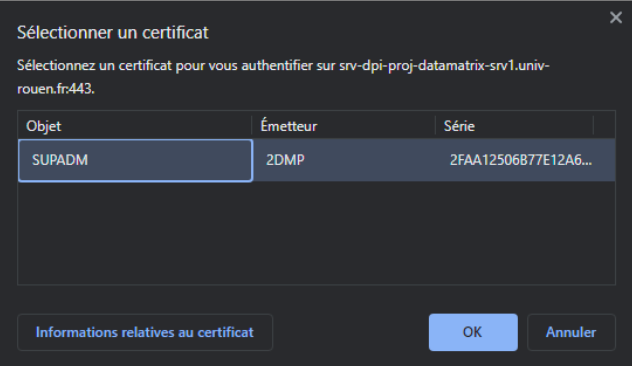
\includegraphics[scale=0.4]{imgs/spadm.PNG}
    \\\texttt{Utilisation du certificat pour s'authentifier}
\end{center}

L'ensemble des procédures de mise en œuvre et des informations techniques sur le principe d'authentification forte \texttt{SSL/TLS} se trouve dans le document \texttt{Doc\Securisation\_Serveur} à la section : \texttt{IV.5. Sécurisation de l’accès à un dossier d’une appli web}, à partir de la sous-section \texttt{IV.5.2. Utilisation d’un certificat}.

\section{Explications Technique}

\subsection{Utilisation de la Base de Données}

En ce qui concerne la base de données, quelques sécurités ont été mises en place. Principalement, l'utilisation de l'API \texttt{PDO} qui permet la mise en place des requêtes préparées. De ce fait, l'ensemble des demandes à la base suivent ce principe afin d'éviter les attaques d'injections.

De plus, l'utilisation de l'algorithme de hachage \texttt{SHA256} est utilisé pour stocker les mots de passe, mais également lors de la vérification. En effet, le mot de passe récupéré est haché et comparé avec le haché stocké.

\begin{center}
    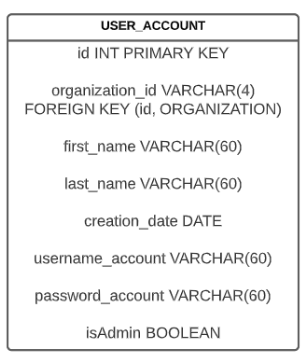
\includegraphics[scale=0.5]{imgs/bd.PNG}\\
    \texttt{Table des comptes dans 2DMATRIX\_DATABASE}
\end{center}
 Pour terminer, on remarque le champ \texttt{isAdmin} contenant le booléen pour distinguer les comptes utilisateur et administrateur.
 
\begin{itemize}
     \item \texttt{vrai} : administrateur organisme
     \item \texttt{faux} : utilisateur organisme
\end{itemize}

Pour avoir des informations complémentaires sur la base de données, vous pouvez regarder le document \texttt{Doc\_Base\_De\_Donnees}.

\subsection{Gestion des sessions PHP}

Les sessions \texttt{PHP} sont activement utilisées par le système d'authentification. 

Par exemple, on utilise la fonction \texttt{session\_regenerate\_id()} à chaque connexion réussie, afin de modifier l'identifiant de session (web) et éviter l'attaque du type \textit{session fixation}. 

Également, à la connexion, on assigne les valeurs de l'identifiant de l'organisme (identifiant donné à la création de quatre caractères) ainsi que le rôle de la personne (\texttt{AdminOrga} ou \texttt{UserOrga}).  

Il y a de nombreuses vérifications au niveau des sessions et en particulier avec la case rôle du tableau de session afin de vérifier que la personne peut accéder à l'URL demandé. Cela permet d'éviter que quelqu'un se connecte par URL sans passer par le système d'authentification.

Pour terminer, les sessions sont détruites à chaque déconnexion (bouton sur les interfaces), ou à chaque passage sur la page d'authentification, pour éviter des problèmes similaires de connexion à des endroits non autorisé via les variables de session et URL.

\end{document}